
\documentclass[12pt]{article}\usepackage[]{graphicx}\usepackage[]{color}
% maxwidth is the original width if it is less than linewidth
% otherwise use linewidth (to make sure the graphics do not exceed the margin)
\makeatletter
\def\maxwidth{ %
  \ifdim\Gin@nat@width>\linewidth
    \linewidth
  \else
    \Gin@nat@width
  \fi
}
\makeatother

\definecolor{fgcolor}{rgb}{0, 0, 0}
\newcommand{\hlnum}[1]{\textcolor[rgb]{0.69,0.494,0}{#1}}%
\newcommand{\hlstr}[1]{\textcolor[rgb]{0.749,0.012,0.012}{#1}}%
\newcommand{\hlcom}[1]{\textcolor[rgb]{0.514,0.506,0.514}{\textit{#1}}}%
\newcommand{\hlopt}[1]{\textcolor[rgb]{0,0,0}{#1}}%
\newcommand{\hlstd}[1]{\textcolor[rgb]{0,0,0}{#1}}%
\newcommand{\hlkwa}[1]{\textcolor[rgb]{0,0,0}{\textbf{#1}}}%
\newcommand{\hlkwb}[1]{\textcolor[rgb]{0,0.341,0.682}{#1}}%
\newcommand{\hlkwc}[1]{\textcolor[rgb]{0,0,0}{\textbf{#1}}}%
\newcommand{\hlkwd}[1]{\textcolor[rgb]{0.004,0.004,0.506}{#1}}%
\let\hlipl\hlkwb

\usepackage{framed}
\makeatletter
\newenvironment{kframe}{%
 \def\at@end@of@kframe{}%
 \ifinner\ifhmode%
  \def\at@end@of@kframe{\end{minipage}}%
  \begin{minipage}{\columnwidth}%
 \fi\fi%
 \def\FrameCommand##1{\hskip\@totalleftmargin \hskip-\fboxsep
 \colorbox{shadecolor}{##1}\hskip-\fboxsep
     % There is no \\@totalrightmargin, so:
     \hskip-\linewidth \hskip-\@totalleftmargin \hskip\columnwidth}%
 \MakeFramed {\advance\hsize-\width
   \@totalleftmargin\z@ \linewidth\hsize
   \@setminipage}}%
 {\par\unskip\endMakeFramed%
 \at@end@of@kframe}
\makeatother

\definecolor{shadecolor}{rgb}{.97, .97, .97}
\definecolor{messagecolor}{rgb}{0, 0, 0}
\definecolor{warningcolor}{rgb}{1, 0, 1}
\definecolor{errorcolor}{rgb}{1, 0, 0}
\newenvironment{knitrout}{}{} % an empty environment to be redefined in TeX

\usepackage{alltt}

\usepackage[hmargin=1in,vmargin=1in]{geometry}
\usepackage{parskip}
\usepackage[hidelinks]{hyperref}
\usepackage{verbatim}



\definecolor{inlinecolor}{rgb}{0.878,0.918,0.933}  
\newcommand{\inr}[1]{\colorbox{inlinecolor}{\texttt{#1}}}







\IfFileExists{upquote.sty}{\usepackage{upquote}}{}
\begin{document}



{
  \Large
  \centering
  {\bf Lab 10 -- Estimating abundance with closed-population capture-mark-recapture data \\ }
  Due before Monday \\
}

\vspace{10pt}


The purpose of this lab is to learn how to estimate abundance using
mark-recapture data from surveys of closed populations. A closed
population does not experience recruitment, mortality, immigration or
emigration. The closure assumption is usually only valid over very
short time periods. We will learn how to work with data from open
populations later.

Work through the problems below, put your code and your answers in a
Word file, and then upload it to ELC. Name the file something like 
``Chandler-lab10.docx''.  

\vspace{-6pt}

\section*{Assignment}

\subsection*{Exercise I: Lincoln-Peterson estimation}

\begin{enumerate}
  \item Suppose you capture, mark, and release 100 largemouth bass ({\it
      Micropterus salmoides}) at Lake Herrick. The next day, you return
    and capture 50 individuals, 25 of which were marked on the first
    occasion. What is the Lincoln-Peterson estimate of abundance ($N$)?
    Do the calculations in R and show your work.
  \item Come up with your own Lincoln-Peterson example like the one
    above, and estimate abundance for a species of your choosing.
    Show your work.
\end{enumerate}



\subsection*{Exercise II: Closed-population models in R}



\begin{enumerate}
  \item Use the R package `mra' to fit the four
    mark-recapture models described in Table~\ref{tab:Otis} to the
    stinkpot ({\it Sternotherus odoratus}) data found in the file
    \texttt{CH-SO-Andy07.inp}. These data were collected using baited
    `hoop traps' at Andy's Pond in 2007. Software instructions are in
    the next section. 
  \item Summarize your results by creating a table in which each row
    is a model, and include the following columns: model description,
    the estimates of $N$ (abundance), the standard errors of $N$ (SE),
    and the AICc values.
  \item Use model $M_t$ to make a graph of capture probability ($p_t$)
    at each time point. You can do this in either Excel or R.
  \item The model with the lowest AICc is considered the best in
    the set of models. Which model has the lowest AICc? Do your
    results suggest that %it is important to account for variation in
    % capture (and recapture) probability over time? Explain.
    there was a behavioral (i.e., a trap-happy or
    trap-shy) response? Explain.
  \item Why do you think model $M_0$ is the worst model
    in the set? Look at the capture histories when answering this
    question. 
  \item Given what you know about turtles and turtle trapping,
    what sources of variation in capture probability (other than time)
    do you think we might want to account for to obtain more reliable
    abundance estimates?
\end{enumerate}

\clearpage

\begin{table}[h!]
  \centering
  \caption{The four models to be fitted to the stinkpot data.}
  \begin{tabular}[h!]{lp{5in}}
    \hline
    Model & Description \\
    \hline
    $M_0$ & The most basic model in which $p$ and $c$ are constant \\
    $M_t$ & $p$ differs among sampling occasions and $p_t=c_t$. \\
    $M_b$ & Behavioral response model in which $p$ and $c$
            differ. Can describe trap happiness or trap shyness. \\
    $M_{tb}$ & A combination of models $M_t$ and $M_b$. \\
    \hline
  \end{tabular}
  \label{tab:Otis}
\end{table}


\vfill



{\bf Parameter definitions}
\begin{itemize}
  \item $p$ -- capture probability. The probability of capturing an
    individual on a single occasion
  \item $p_t$ -- capture probability on occasion $t$
  \item $c$ -- recapture probability. The probability of capturing an
    individual that has been captured previously.
  \item $n$ -- the number of individuals captured
  \item $f_0$ -- the number of individual not captured
  \item $N$ -- abundance. The number of individuals in the
    population. $N=n+f_0$. 
\end{itemize}

\vfill


\begin{figure}[h!]
  \centering
  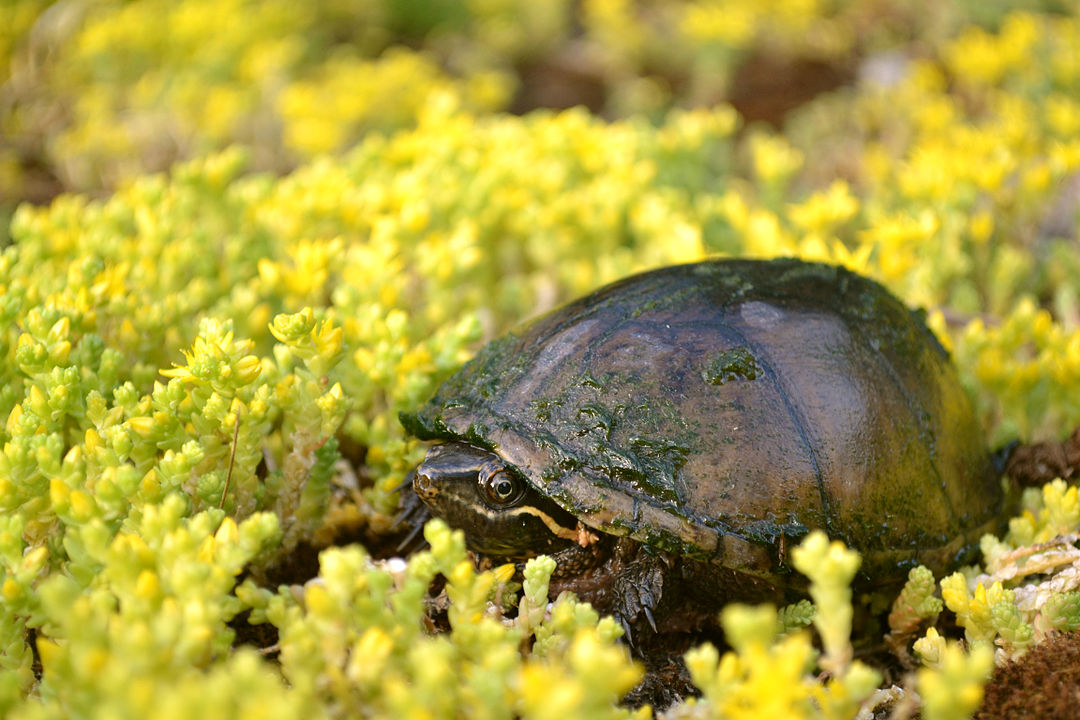
\includegraphics[width=0.7\textwidth]{figs/Stinkpot} \\
  \caption{A stinkpot}
\end{figure}



\clearpage


\section*{Example analysis in R}

Open R (or RStudio) and install the ``mra'' package using the
following command: 

\begin{knitrout}
\definecolor{shadecolor}{rgb}{0.878, 0.918, 0.933}\color{fgcolor}\begin{kframe}
\begin{alltt}
\hlkwd{install.packages}\hlstd{(}\hlstr{"mra"}\hlstd{)}
\end{alltt}
\end{kframe}
\end{knitrout}

Now load the package like so: 

\begin{knitrout}
\definecolor{shadecolor}{rgb}{0.878, 0.918, 0.933}\color{fgcolor}\begin{kframe}
\begin{alltt}
\hlkwd{library}\hlstd{(mra)}
\end{alltt}
\end{kframe}
\end{knitrout}

The example bear data are formatted for program MARK, but we can
import them using  \inr{read.table}. The only trick is to tell R that
the capture histories should be treated as a character string, rather
than as a numeric variable. The \inr{colClasses} arguments let's us do
that. 

\begin{knitrout}
\definecolor{shadecolor}{rgb}{0.878, 0.918, 0.933}\color{fgcolor}\begin{kframe}
\begin{alltt}
\hlstd{capture.histories} \hlkwb{<-} \hlkwd{read.table}\hlstd{(}\hlstr{"CH-example.inp"}\hlstd{,} \hlkwc{sep}\hlstd{=}\hlstr{" "}\hlstd{,}
                                \hlkwc{colClasses}\hlstd{=}\hlkwd{c}\hlstd{(}\hlstr{"character"}\hlstd{,} \hlstr{"character"}\hlstd{),}
                                \hlkwc{col.names}\hlstd{=}\hlkwd{c}\hlstd{(}\hlstr{"ch"}\hlstd{,} \hlstr{"freq"}\hlstd{))}
\end{alltt}
\end{kframe}
\end{knitrout}

%                                #"CH-SO-Andy07.inp", sep=" ",


It's a small dataset, so we can display it in full:

\begin{knitrout}
\definecolor{shadecolor}{rgb}{0.878, 0.918, 0.933}\color{fgcolor}\begin{kframe}
\begin{alltt}
\hlstd{capture.histories}
\end{alltt}
\begin{verbatim}
##        ch freq
## 1  101001   1;
## 2  100001   1;
## 3  100001   1;
## 4  010000   1;
## 5  101000   1;
## 6  010001   1;
## 7  001000   1;
## 8  001011   1;
## 9  000100   1;
## 10 001001   1;
## 11 001000   1;
## 12 000010   1;
## 13 000010   1;
## 14 000101   1;
\end{verbatim}
\end{kframe}
\end{knitrout}


We need to convert the capture histories from a character vector to a
matrix. The following code does the trick.


\begin{knitrout}
\definecolor{shadecolor}{rgb}{0.878, 0.918, 0.933}\color{fgcolor}\begin{kframe}
\begin{alltt}
\hlstd{ch.mat} \hlkwb{<-} \hlkwd{t}\hlstd{(}\hlkwd{sapply}\hlstd{(capture.histories}\hlopt{$}\hlstd{ch,}
                   \hlkwa{function}\hlstd{(}\hlkwc{x}\hlstd{)} \hlkwd{as.integer}\hlstd{(}\hlkwd{strsplit}\hlstd{(x,} \hlstr{""}\hlstd{)[[}\hlnum{1}\hlstd{]])))}
\hlkwd{dimnames}\hlstd{(ch.mat)} \hlkwb{<-} \hlkwd{list}\hlstd{(}\hlkwd{paste0}\hlstd{(}\hlstr{"Bear"}\hlstd{,} \hlnum{1}\hlopt{:}\hlkwd{nrow}\hlstd{(capture.histories)),}
                         \hlkwd{paste0}\hlstd{(}\hlstr{"Time"}\hlstd{,} \hlnum{1}\hlopt{:}\hlnum{6}\hlstd{))}
\end{alltt}
\end{kframe}
\end{knitrout}


\clearpage

Now the capture histories look like this:

\begin{knitrout}
\definecolor{shadecolor}{rgb}{0.878, 0.918, 0.933}\color{fgcolor}\begin{kframe}
\begin{alltt}
\hlstd{ch.mat}
\end{alltt}
\begin{verbatim}
##        Time1 Time2 Time3 Time4 Time5 Time6
## Bear1      1     0     1     0     0     1
## Bear2      1     0     0     0     0     1
## Bear3      1     0     0     0     0     1
## Bear4      0     1     0     0     0     0
## Bear5      1     0     1     0     0     0
## Bear6      0     1     0     0     0     1
## Bear7      0     0     1     0     0     0
## Bear8      0     0     1     0     1     1
## Bear9      0     0     0     1     0     0
## Bear10     0     0     1     0     0     1
## Bear11     0     0     1     0     0     0
## Bear12     0     0     0     0     1     0
## Bear13     0     0     0     0     1     0
## Bear14     0     0     0     1     0     1
\end{verbatim}
\end{kframe}
\end{knitrout}

We will use the \inr{F.huggins.estim} function to fit the
closed population models. Model $M_0$ can be fit like this: 

\begin{knitrout}
\definecolor{shadecolor}{rgb}{0.878, 0.918, 0.933}\color{fgcolor}\begin{kframe}
\begin{alltt}
\hlstd{M0} \hlkwb{<-} \hlkwd{F.huggins.estim}\hlstd{(}\hlkwc{capture}\hlstd{=}\hlopt{~}\hlnum{1}\hlstd{,} \hlkwc{recapture}\hlstd{=}\hlkwa{NULL}\hlstd{,} \hlkwc{histories}\hlstd{=ch.mat)}
\end{alltt}
\end{kframe}
\end{knitrout}

Model $M_b$ like this:

\begin{knitrout}
\definecolor{shadecolor}{rgb}{0.878, 0.918, 0.933}\color{fgcolor}\begin{kframe}
\begin{alltt}
\hlstd{Mb} \hlkwb{<-} \hlkwd{F.huggins.estim}\hlstd{(}\hlkwc{capture}\hlstd{=}\hlopt{~}\hlnum{1}\hlstd{,} \hlkwc{recapture}\hlstd{=}\hlopt{~}\hlnum{1}\hlstd{,} \hlkwc{histories}\hlstd{=ch.mat)}
\end{alltt}
\end{kframe}
\end{knitrout}

To fit model $M_t$, we have to create a time variable.

\begin{knitrout}
\definecolor{shadecolor}{rgb}{0.878, 0.918, 0.933}\color{fgcolor}\begin{kframe}
\begin{alltt}
\hlstd{time} \hlkwb{<-} \hlkwd{tvar}\hlstd{(}\hlkwd{factor}\hlstd{(}\hlnum{1}\hlopt{:}\hlnum{6}\hlstd{),} \hlkwc{nan}\hlstd{=}\hlkwd{nrow}\hlstd{(ch.mat))} \hlcom{## 6 time periods. 14 animals.}
\hlstd{Mt} \hlkwb{<-} \hlkwd{F.huggins.estim}\hlstd{(}\hlkwc{capture}\hlstd{=}\hlopt{~}\hlstd{time,} \hlkwc{recapture}\hlstd{=}\hlkwa{NULL}\hlstd{,} \hlkwc{histories}\hlstd{=ch.mat)}
\end{alltt}
\end{kframe}
\end{knitrout}


You should be able to figure out how to fit model $M_{tb}$ by
extending the code above.

\clearpage

Estimates of abundance along with AICc values can be found by typing
the name of the fitted model object. For example:

\begin{knitrout}
\definecolor{shadecolor}{rgb}{0.878, 0.918, 0.933}\color{fgcolor}\begin{kframe}
\begin{alltt}
\hlstd{M0}
\end{alltt}
\begin{verbatim}
## Call:
## F.huggins.estim(capture = ~1, recapture = NULL, histories = ch.mat)
## 
##  Capture and Recapture model:
##  Variable     Est       SE     
##  (Intercept)  -1.25004  0.32308 
## 
## Population Size Estimate (se): 17.962 (3.1462)
## 95% confidence interval for population size: 15.01 to 29.6
## Individuals observed: 14
## Effective sample size: 84
## 
## Message =  SUCCESS: Convergence criterion met
## Number of estimable coefficients (estimated) =  1
## Log likelihood =  -47.6734852287387
## Deviance =  95.3469704574774
## AIC =  97.3469704574774
## AICc =  97.3957509452822
\end{verbatim}
\end{kframe}
\end{knitrout}


You can extract the capture probability estimates for each individual
on each sampling occasion:

\begin{knitrout}
\definecolor{shadecolor}{rgb}{0.878, 0.918, 0.933}\color{fgcolor}\begin{kframe}
\begin{alltt}
\hlkwd{round}\hlstd{(M0}\hlopt{$}\hlstd{p.hat,} \hlkwc{digits}\hlstd{=}\hlnum{3}\hlstd{)}
\end{alltt}
\begin{verbatim}
##        [,1]  [,2]  [,3]  [,4]  [,5]  [,6]
##  [1,] 0.223 0.223 0.223 0.223 0.223 0.223
##  [2,] 0.223 0.223 0.223 0.223 0.223 0.223
##  [3,] 0.223 0.223 0.223 0.223 0.223 0.223
##  [4,] 0.223 0.223 0.223 0.223 0.223 0.223
##  [5,] 0.223 0.223 0.223 0.223 0.223 0.223
##  [6,] 0.223 0.223 0.223 0.223 0.223 0.223
##  [7,] 0.223 0.223 0.223 0.223 0.223 0.223
##  [8,] 0.223 0.223 0.223 0.223 0.223 0.223
##  [9,] 0.223 0.223 0.223 0.223 0.223 0.223
## [10,] 0.223 0.223 0.223 0.223 0.223 0.223
## [11,] 0.223 0.223 0.223 0.223 0.223 0.223
## [12,] 0.223 0.223 0.223 0.223 0.223 0.223
## [13,] 0.223 0.223 0.223 0.223 0.223 0.223
## [14,] 0.223 0.223 0.223 0.223 0.223 0.223
\end{verbatim}
\end{kframe}
\end{knitrout}

For model $M_0$, capture probability is the same for all individuals
during all time periods. This won't be the case for the other models. 




\end{document}




